\documentclass[../Thesis.tex]{subfiles}
\begin{document}
	
	\chapter{State of the Art}
	\label{sec:state_of_the_art_review}
	
	Calculating the GED with traditional imperative algorithm is possible but feasible only for graphs of modest size. GED is a NP-HARD problem and for traditional solutions there is no way except to compare graphs node by node and edge by edge through combinatorial techniques to find a solution. However, as the number of nodes in the graphs increase, the time needed by these methods grows exponentially, leading to scalability issues thus infeasibility. To overcome these limitations recent works involve the use of artificial intelligence techniques such as neural networks to predict the GED between two graphs. AI-based approaches usually offer more robust and scalable solutions by learning patterns and features from graphs, significantly reducing computation times. This section reviews some of the most important papers dealing with GED calculation from 2019 to the time of writing this (2024).

	A timeline of significant works, beginning in 2019 with \textit{SimGNN} \cite{simgnn__a_neural_network_approach_to_fast_graph_similarity_computation}, the first to use neural networks for GED computation, is discussed in \autoref{sec:timeline}. Following \textit{SimGNN}, numerous models have been developed, each trying to offer something new and better performances. The timeline concludes with the most recent and promising model, \textit{GedGNN} \cite{computing_graph_edit_distance_via_neural_graph_matching}. Although these models strive to estimate GED between graphs accurately, as will be shown, this area is still in the early stages of development.
	
	
	\section{Timeline}
	\label{sec:timeline}
        \quad
 
	2019, \textit{SimGNN: A Neural Network Approach to Fast Graph Similarity Computation} \cite{simgnn__a_neural_network_approach_to_fast_graph_similarity_computation}: Presents the SimGNN to solve the problem of graph similarity using neural networks. It uses a learnable embedding function, an attention mechanism to capture important nodes, and a pairwise node comparison, which is more general and efficient than the baselines.
	
	2020, \textit{Learning Graph Edit Distance by Graph Neural Networks} \cite{learning_graph_edit_distance_by_graph_neural_networks}: Presents a framework that integrates deep metric learning with the conventional approximations of graph edit distance using geometric deep learning. The approach uses a message passing neural network (MPNN) to encode graph structure and compute graph distances effectively, achieving state-of-the-art performance in graph retrieval and competitive results in graph similarity learning.
	
	2020, \textit{Combinatorial Learning of Graph Edit Distance via Dynamic Embedding} \cite{combinatorial_learning_of_graph_edit_distance_via_dynamic_embedding}: Proposes a new method to solve the GED problem through a combination of dynamic graph embedding network and an edit path search method to improve the interpretability and the efficiency of the approach. The learning-based A* algorithm decreases the size of the search tree and time while providing a minor decrease in the solution quality.
	
	2021, \textit{Graph Partitioning and Graph Neural Network-Based Hierarchical Graph Matching for Graph Similarity Computation} \cite{graph_partitioning_and_graph_neural_network_based_hierarchical_graph_matching_for_graph_similarity_computation}: Presents PSimGNN that first divides input graphs into subgraphs to learn local structural patterns and then employs a new GNN with attention to map subgraphs to embeddings and then combines coarse-grained interaction between subgraphs with fine-grained node-wise comparison to estimate similarity scores.
	
	2021, \textit{Noah: Noah: Neural Optimized A* Search Algorithm for Graph Edit Distance Computation} \cite{noah__neural_optimized_a*_search_algorithm_for_graph_edit_distance_computation}: Presents Noah that uses A* search and GPN for approximate GED calculation. Noah estimates the cost function using GPN, includes pre-training with attention-based information, and uses an elastic beam size to decrease the search space.
	
	2021, \textit{Learning Efficient Hash Codes for Fast Graph-Based Data Similarity Retrieval} \cite{learning_efficient_hash_codes_for_fast_graph_based_data_similarity_retrieval}: Proposes HGNN (Hash Graph Neural Network) that is a model for efficient graph-based data retrieval using GNNs and hash learning algorithms. HGNN learns a similarity-preserving graph representation and then generates short hash codes for efficient retrieval and classification.
	
	2021, \textit{More Interpretable Graph Similarity Computation via Maximum Common Subgraph Inference} \cite{more_interpretable_graph_similarity_computation_via_maximum_common_subgraph_inference}: Presents INFMCS, an end-to-end framework for graph similarity learning with an interpretable similarity score that is based on the correlation between the score and the Maximum Common Subgraph (MCS), and combines transformer encoder layers with graph convolution for high accuracy and interpretability.
	
	2021, \textit{H2MN: Graph Similarity Learning with Hierarchical Hypergraph Matching Networks} \cite{h2mn__graph_similarity_learning_with_hierarchical_hypergraph_matching_networks}: Presents H2MN, which computes the similarity of graph-structured data by converting graphs to hypergraphs and performing subgraph matching at the hyperedge level, and then a multi-perspective cross-graph matching layer.
	
	2022, \textit{TaGSim: Type-aware Graph Similarity Learning and Computation} \cite{TaGSim_type_aware_graph_similarity_learning_and_computation}: This work introduces TaGSim, a type-aware graph similarity learning and computation approach that overcomes the drawbacks of traditional GED methods by incorporating type-specific graph edit operations. TaGSim models the effects of various graph modifications (node and edge insertions, deletions, and relabelings) as separate operations, which generate type-aware embeddings and use them for estimating the GED. The framework outperforms other GED solutions on real-world datasets as shown in the framework.
	
	2023, \textit{Efficient Graph Edit Distance Computation Using Isomorphic Vertices} \cite{efficient_graph_edit_distance_computation_using_isomorphic_vertices}: Introduces a new strategy for the reduction of the search space of GED computation through the identification of isomorphic vertices, aiming at the elimination of unnecessary vertex mappings and thus a substantial reduction of the computation time for exact GED.
	
	2023, \textit{Exploring Attention Mechanism for Graph Similarity Learning} \cite{exploring_attention_mechanism_for_graph_similarity_learning}: Introduces a single model with attention mechanisms for node embedding, cross-graph co-attention for interaction modeling, and graph similarity matrix learning for score prediction and outperforms the state of the art on benchmark datasets.
	
	2023, \textit{Graph Edit Distance Learning via Different Attention} \cite{graph_edit_distance_learning_via_different_attention}: Proposes DiffAtt, a new graph-level fusion module for GNNs to compute GED efficiently with the help of structural differences between graphs using attention, integrated into the GSC model REDRAFT, which outperforms the state of the art on benchmark datasets.
	
	2023, \textit{Graph-Graph Context Dependency Attention for Graph Edit Distance} \cite{graph_graph_context_dependency_attention_for_graph_edit_distance}: Presents GED-CDA, a deep network architecture for GED computation which uses a graph-graph context dependency attention module that combines cross-attention and self-attention layers to model inter-graph and intra-graph dependencies.
	
	2023, \textit{GREED: A Neural Framework for Learning Graph Distance Functions}: Introduces GREED, a siamese GNN for learning GED and SED in a property preserving manner which outperforms other methods in terms of accuracy and time complexity.
	
	2023, \textit{MATA*: Learnable Node Matching with A* Algorithm for Approximate Graph Edit Distance} \cite{mata_combining_learnable_node_matching_with_a*_algorithm_for_approximate_graph_edit_distance}: Presents MATA*, a novel approach for the approximate GED computation that combines GNNs and the A* algorithm, with the focus on learning the node matching.
	
	2023, \textit{Multilevel Graph Matching Networks for Deep Graph Similarity Learning} \cite{multilevel_graph_matching_networks_for_deep_graph_similarity_learning}: Introduces MGMN, a multilevel graph matching network that can capture the cross-level interactions, which includes NGMN and a siamese GNN for global-level interactions, and performs well when graph sizes are large.
	
	2023, \textit{Wasserstein Graph Distance Based on L1-Approximated Tree Edit Distance Between Weisfeiler-Lehman Subtrees} \cite{wasserstein_graph_distance_based_on_l1_approximated_tree_edit_distance_between_weisfeiler_lehman_subtrees}: Introduces the WWLS distance which integrates WL subtrees with L1-TED which is more sensitive to fine changes in the structure of graphs and outperforms other methods in metric validation and graph classification.
	
	2023, \textit{Computing Graph Edit Distance via Neural Graph Matching} \cite{computing_graph_edit_distance_via_neural_graph_matching}: Presents GEDGNN, a deep learning model for GED computation that works on the idea of graph transformation instead of directly predicting GED value. GEDGNN provides GED values and a matching matrix and a post-processing procedure for obtaining high quality node mappings.

\section{Trends in the field of GNN-based GED approximation}
The previous timeline shows that the field of graph similarity and graph edit distance (GED) computation has evolved significantly from 2019 to 2023, with most approaches building upon the Siamese Graph Neural Network architecture by adding various layers and operations. Techniques such as SimGNN\cite{simgnn__a_neural_network_approach_to_fast_graph_similarity_computation} and subsequent models typically enhance neural networks with additional layers, like attention mechanisms\cite{simgnn__a_neural_network_approach_to_fast_graph_similarity_computation, noah__neural_optimized_a*_search_algorithm_for_graph_edit_distance_computation, exploring_attention_mechanism_for_graph_similarity_learning, graph_edit_distance_learning_via_different_attention, graph_graph_context_dependency_attention_for_graph_edit_distance}, Graph Isomorphism Networks (GIN) \cite{noah__neural_optimized_a*_search_algorithm_for_graph_edit_distance_computation}, message passing neural networks \cite{learning_graph_edit_distance_by_graph_neural_networks}, or by leveraging hierarchical structures through graph partitioning and hypergraph matching \cite{graph_partitioning_and_graph_neural_network_based_hierarchical_graph_matching_for_graph_similarity_computation, multilevel_graph_matching_networks_for_deep_graph_similarity_learning, h2mn__graph_similarity_learning_with_hierarchical_hypergraph_matching_networks}. These layers help in capturing intricate details of graph structures and improving efficiency and accuracy in similarity computations. However, some approaches stand out due to their distinct methodologies. For instance, TaGSim \cite{TaGSim_type_aware_graph_similarity_learning_and_computation} incorporates type-specific graph edit operations and synthetic data generation. Additionally, approaches such as Noah\cite{noah__neural_optimized_a*_search_algorithm_for_graph_edit_distance_computation} and MATA*\cite{mata_combining_learnable_node_matching_with_a*_algorithm_for_approximate_graph_edit_distance} combine neural networks with classical algorithms like the A* search, showcasing innovative blends of traditional and modern techniques. These unique strategies highlight the diversity and depth of research efforts aimed at enhancing graph similarity and GED computations, inspiring state of the art approaches such as \cite{computing_graph_edit_distance_via_neural_graph_matching}.

Following the choice of model which inspired the current state of the art, GedGNN\cite{computing_graph_edit_distance_via_neural_graph_matching}, in the following sections the following four models, SimGNN\cite{simgnn__a_neural_network_approach_to_fast_graph_similarity_computation}, GPN\cite{noah__neural_optimized_a*_search_algorithm_for_graph_edit_distance_computation}, TaGSim\cite{TaGSim_type_aware_graph_similarity_learning_and_computation}, and GedGNN\cite{computing_graph_edit_distance_via_neural_graph_matching} will be described in more detail.
	
	\section{SimGNN}
	\label{sec:simgnn}
	
	The first innovative model that used neural networks is SimGNN \cite{simgnn__a_neural_network_approach_to_fast_graph_similarity_computation}, introduced in 2019. SimGNN serves as a foundational model in the field of graph similarity computation, in fact future models will often inherit its core concepts (such as the siamese layout architecture), making it the starting point of reference for anyone dealing with GED computation. 
	
	The architecture of SimGNN [\autoref{fig:simgnn_architecture}] is composed by several stages:
	
	\begin{itemize}
		\item \textbf{Node Embedding Stage}: This stage makes use of a graph convolutional network to capture local structural information that transforms each node in the graph into a vector that encodes its features and structural properties.
		\item \textbf{Graph-Level Embedding Stage}: This stage produces a single embedding representing the whole graphs starting from the previously produced nodes embeddings by also using attention mechanisms to focus on important nodes.
		\item \textbf{Graph-Graph Interaction Stage}: This stage puts in communication the two graphs embedding previously produced and produces a matrix of similarity interaction scores.
		\item \textbf{Final Similarity Score Computation Stage}: This stage process the previously produced similarity matrix to compute the final similarity score.
	\end{itemize}
	
	In addition to the graph-level embedding interaction strategy, SimGNN has a its disposal a pairwise node comparison strategy:
	
	\begin{itemize}
		\item \textbf{Pairwise Node Comparison}: This strategy involves computing pairwise interaction scores between the node embeddings of the two graphs. The resulting similarity matrix is used to extract histogram features, which are then combined with the graph-level interaction scores to provide a comprehensive view of graph similarity.
	\end{itemize}
	
	The combination of these two strategies should allow the model to capture both global and local informations which should result in a robust approach to graph similarity computation.
	
	\begin{figure}[H]
		\centering
		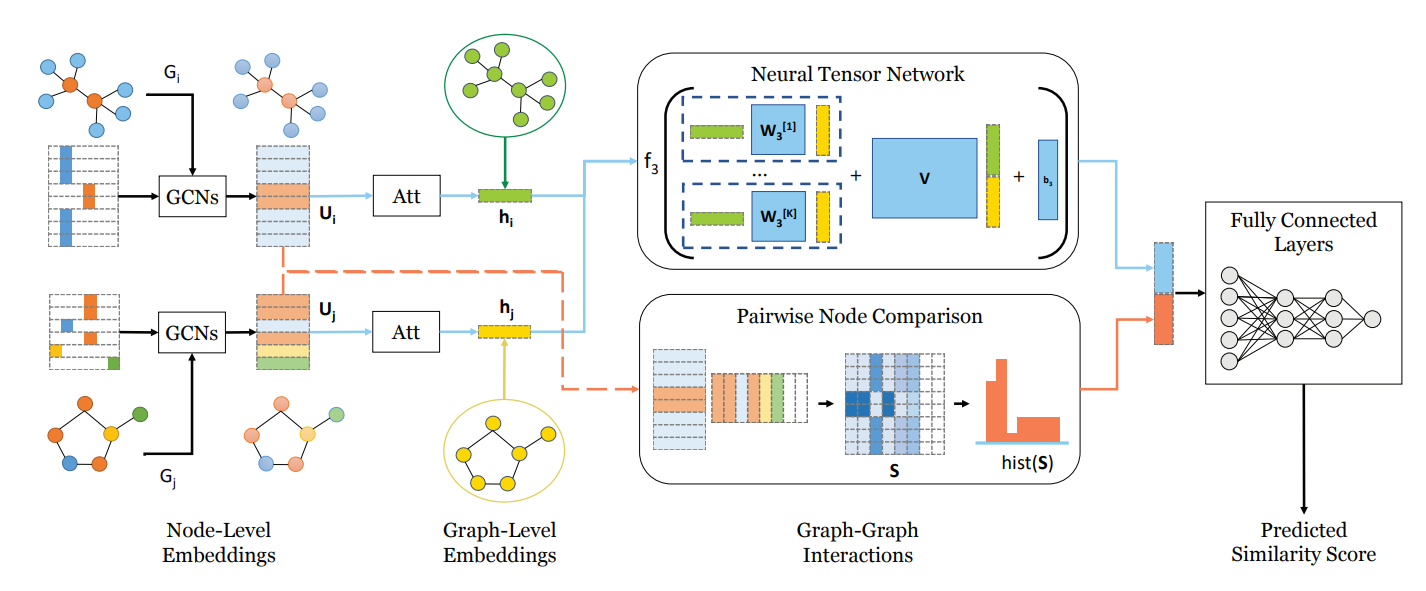
\includegraphics[width=\textwidth]{Images/simgnn_architecture.png}
		\caption{SimGNN architecture overview taken from \cite{simgnn__a_neural_network_approach_to_fast_graph_similarity_computation}.}
		\label{fig:simgnn_architecture}
	\end{figure}

	
	\section{GPN}
	\label{sec:gpn}
	
	In 2022, an innovative hybrid approach for computing GED was released.
	The Graph Path Networks (GPN) model, proposed within the \textit{NOAH Framework} \cite{noah__neural_optimized_a*_search_algorithm_for_graph_edit_distance_computation}, introduces the GED computation by exploiting the A* search algorithm optimized through neural networks. This method tries to address several previously found limitations trying to improve both the search direction and search space optimization.
	
	The architecture of GPN [\autoref{fig:gpn_architecture}] is composed by several modules:
	
	\begin{itemize}
		\item \textbf{Pre-training Module}: This module computes pre-training information about the graphs that will be exploited by the next modules.
		\item \textbf{Graph Embedding Module}: This module utilizes layers of Graph Isomorphism Network (GIN) to transform each node into a vector. Then these embeddings are combined into a single graph level embedding by using different attention mechanisms.
		\item \textbf{Learning Module}: This module focuses on optimizing the A* search algorithm by learning an estimated cost function and an elastic beam size. The tradition algorithm is then used for the final prediction.
	\end{itemize}
	
	The main advantage of GPN over SimGNN is that it is capable of finding an edit path between graphs (roughly accurate) between graphs in a short amount of time.
	
	\begin{figure}[H]
		\centering
		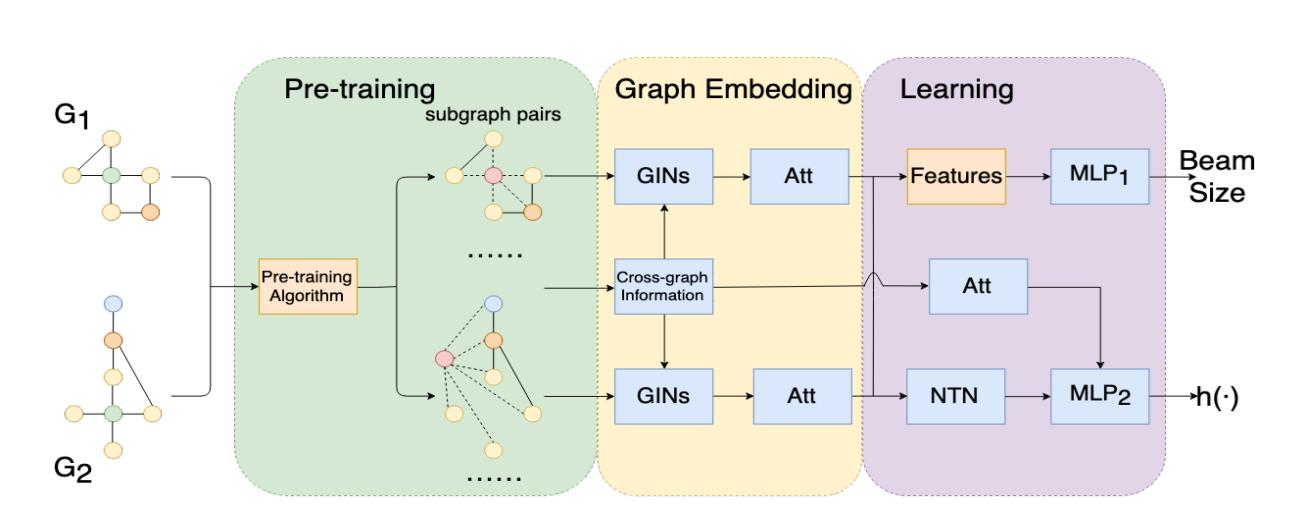
\includegraphics[width=\textwidth]{Images/gpn_architecture.png}
		\caption{GPN architecture overview taken from \cite{noah__neural_optimized_a*_search_algorithm_for_graph_edit_distance_computation}.}
		\label{fig:gpn_architecture}
	\end{figure}
	
	
	\section{TaGSim}
	\label{sec:tagsim}
	
	In 2022, another innovative approach was released with TaGSim (Type-aware Graph Similarity) \cite{TaGSim_type_aware_graph_similarity_learning_and_computation}. The idea behind GED as a single value has been revaluated and it is now thought as the summation of three different values: $ged\_nc$ the number of node relabelling, $ged\_in$ the number of node insertions/deletions, $ged\_ie$ the number of edges insertions/deletions. 
	
	The architecture of TaGSim [\autoref{fig:tagsim_architecture}] is composed by several components:
	
	\begin{itemize}
		\item \textbf{Type-Aware Graph Embeddings}: This component takes into account the different impacts that different atomic operations could have when predicting the GED producing a type-aware graph level embedding. Namely the operations taken into accounts are: node insertion/deletion (NR), node relabeling (NID), edge insertion/deletion (ER), and edge relabeling (EID). Each type of operation is handled separately to capture its localized effects on the graph.
		\item \textbf{Type-Aware Neural Networks}: This component takes advantage of specific neural networks that are specifically designed to process and learn from the type-aware embeddings. This allows TaGSim to achieve high accuracy in GED estimation by incorporating the distinct impacts of different edit types and outputs them all.
	\end{itemize}
	
	The main advantage of TaGSim over predecessors is that by decoupling the GED into different dimensions, there is the potential for more granular control and learnability.
	
	\begin{figure}[H]
		\centering
		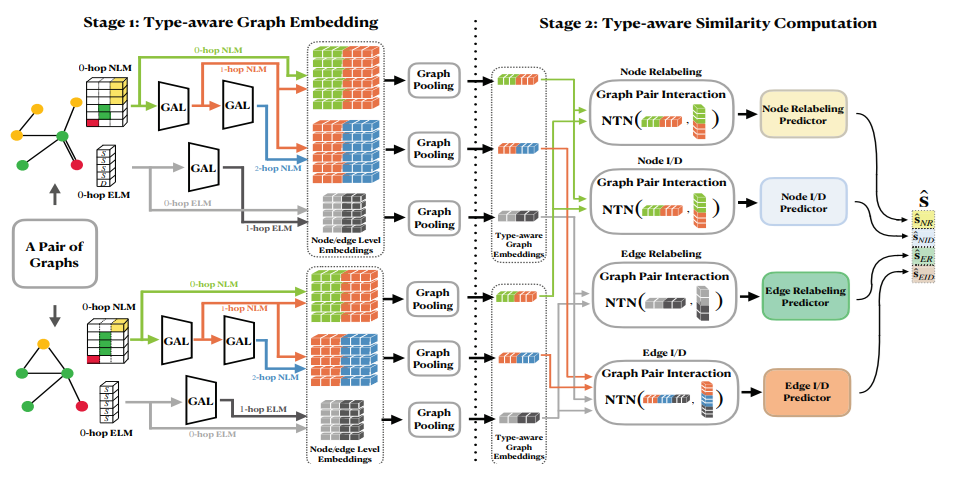
\includegraphics[width=\textwidth]{Images/tagsim_architecture.png}
		\caption{TaGSim architecture overview taken from \cite{TaGSim_type_aware_graph_similarity_learning_and_computation}.}
		\label{fig:tagsim_architecture}
	\end{figure}

	\section{GedGNN}
	\label{sec:gedgnn}
	
	In 2023, the model that is considered the state of the art at the time of writing this (2024) is released with GedGNN (Graph Edit Distance via Neural Graph Matching) \cite{computing_graph_edit_distance_via_neural_graph_matching}. The idea behind this model is to try to put together all the best ideas from past's models including the basic siamese layout of SimGNN, the use of more advanced convolutional layers of GPN and the split of the GED metric from TaGSim while still allowing for the retrieval of an edit paths by taking inspiration from NOAH framework.
	
	The architecture of GedGNN [\autoref{fig:gedgnn_architecture}] is composed by several components:
	
	\begin{itemize}
		\item \textbf{Graph Neural Network (GNN) Encoder}: This component produces the encodings for nodes and edges while preserving their relational information. This is done through the employment of an advanced GNN encoder.
		\item \textbf{Node and Edge Matching Module}: This component performs the node and edge matching between the pair of graphs producing a matching matrix and a cost matrix.
		\item \textbf{k-Best Matching Post-Processing Algorithm}: After predicting the GED value a k-best post-processing algorithm is used trying to retrieve a good edit path.
	\end{itemize}
	
	GedGNN's results state to not only outperforms previous methods but also provides a flexible framework that can adapt to various types of graph structures and similarity measures.
	
	\begin{figure}[H]
		\centering
		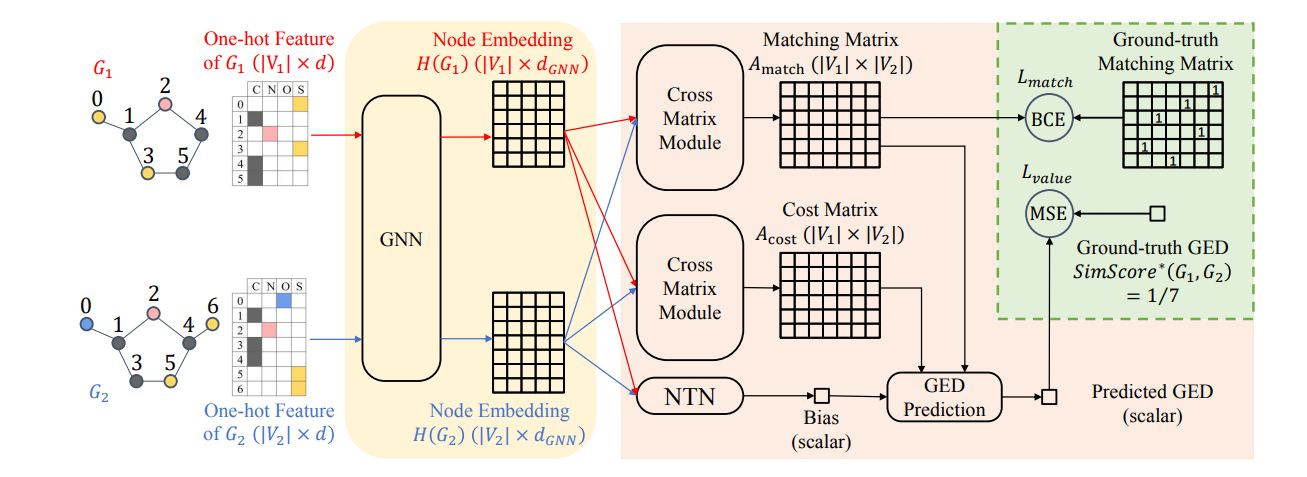
\includegraphics[width=\textwidth]{Images/gedgnn_architecture.png}
		\caption{GedGNN architecture overview taken from \cite{computing_graph_edit_distance_via_neural_graph_matching}.}
		\label{fig:gedgnn_architecture}
	\end{figure}
	
\section{Identified issues in the GedGNN codebase}
\label{sec:issues-codebase}

 In this research, several problems and concerns have been identified within the \href{https://github.com/ChengzhiPiao/GEDGNN}{codebase of GedGNN}.

\begin{description}
    \item[Code Quality:] The GedGNN codebase was found to be fragile, difficult to extend and not well documented. There are numerous redundant method implementations, an excess of classes, and insufficient error handling. This makes it difficult to extend it with other models or variations in the workflow. In fact, in some instances, the code appears almost hard-coded and brittle. For example, the original code does not allow for training a model on one dataset and then testing it on another, thus preventing testing for out-of-distribution generalization. Additionally, the code expects the input to be a matrix of distances between graph couples, making it difficult to test on other datasets that do not follow this format.
    \item[Scalability on GPUs:] The codebase also faces issues with scalability on GPUs. When attempting to run the code on a GPU for the first time, errors often arise. Moreover, the models do not scale well on GPU hardware. While training on small datasets is feasible on CPUs, using large datasets for training new models leads to long training times per epoch, posing a significant challenge.
    \item[Graph Size Limitation:] The codebase only supports graphs with 10 nodes or fewer in training, testing, and validation scenarios. This limitation may be due to the complex algorithms used, such as the k-best post-processing algorithm for reconstructing edit paths. Additionally, the code fails when tested on the IMDB dataset. Despite the presence of artificial dataset generation code, it is not utilized, resulting in confusion and unreachable code paths.
    \item[Training Data Issues:] High-quality data is crucial for the performance of deep learning models. However, the training data issues date back to the creation of SimGNN. The same small datasets, containing graphs with fewer than ten nodes, are reused repeatedly. The primary concern is that approximate GEDs are used as labels instead of exact ones, making the learned model an approximation of the approximation. For graphs of this size, calculating the GED exactly would be better and feasible. Additionally, the use of synthetic data, where graphs at known GEDs are synthetically generated, has not been seriously considered.
    \item[Fair Testing Between Models:] The most significant problem is the lack of fair testing between models. Currently, models are tested by training them on each dataset and testing them on the respective test set of each dataset. This approach, at best, tests for in-distribution generalization but fails to test for out-of-distribution generalization. Out-of-distribution generalization is the ability of a model to perform well when tested with examples that are sufficiently different from those on which it was trained.
\end{description}

In summary, the analyzed codebase for GedGNN, TaGSim, SimGNN, and GPN present several significant challenges. These include issues with reproducibility of results, fair evaluations, scalability, poor code quality, and unclear parameters. Addressing these issues would significantly advance this field and improve the reliability and usability of these models.
	
\end{document}
